% Thesis: Nomadic Time
% Author: Andrew Hughes

\chapter{Nomadic Time}
\label{nt}

\section{Introduction}

This chapter introduces the process calculus used as the basis for
DynamiTE, Nomadic Time.  Over the course of the first half of this
chapter, we show how CaSE (itself a derivative of CCS) is extended
with first localities (see \ref{localising}) and then mobility (see
\ref{addingmob}) to create a calculus which provides both the ability
to migrate processes during execution and to perform global
synchronisation in a compositional manner.  We then introduce the
concept of `bouncers' (see \ref{bouncers}), which allow migration to
be restricted; they define which mobility actions may be performed and
how many times.  This is followed by the operational semantics of the
calculus (see \ref{ntsemantics}).  Finally, we close with a
comprehensive example (see \ref{example}) demonstrating each feature
of the calculus and the application of the calculus to our
prototypical application (see \ref{app:nt}).

\section{Localising the Calculus}
\label{localising}

\emph{Localisation}, discussed in detail in \ref{migration}, effectively
adds another level of grouping to the calculus.  A set of composed
processes may be contained within one \emph{locality}, a notion which is
often used in the modelling of \emph{distribution}.  This idea, which
can be taken to its logical conclusion by forming a hierarchy of such
localities, has echoes of the notion of \emph{clock hiding} within CaSE,
as just described.

Thus, the first step in the evolution towards NT is to combine these
two hierarchical concepts by effectively localising CaSE.  The notion of
components and encapsulation is explicitly realised by an
\emph{environ}, which also handles the hiding of clocks.  As a result,
the clock hiding operator from CaSE disappears, being replaced by a new
operator which allows the creation of environs.  The bounds of the
environ define both a new group and the scope of the clock hiding.  The
syntax for localised CaSE is thus:
\begin{equation}
  \begin{aligned}
    \expr, \exprb\ ::=\ &
    \nil  \;\,|\,\; 
    \Delta \;\,|\,\; 
    \Delta_{\sigma} \;\,|\,\; 
    \alpha . \expr  \;\,|\,\;
    \expr + \exprb \;\,|\,\; 
    (\expr\;|\;\exprb)\;\,|\,\; 
    \timeout{\expr}{\sigma}{\exprb} \;\,|\,\; \\
    & \stimeout{\expr}{\sigma}{\exprb} \;\,|\,\; 
    \mu X . \expr \;\,|\,\; 
    X \;\,|\,\; 
    \expr \setminus a \;\,|\,\; 
    \lclocv{m}{\expr}{\vec{\sigma}}
  \end{aligned}
\end{equation}
where $m$ represents an arbitrary environ name\footnote{Note
that although names are added to the environs here, this is not really
necessary at this stage; they provide nothing more than a way to refer
to environs in talking about a system.  However, they are necessary
for providing migration as discussed in \ref{migration}}.  In
particular, $m$ may be equal to the empty string, $\epsilon$, thus
facilitating the use of anonymous environs.  This allows the semantics
of CaSE's clock hiding to be encoded:

\begin{equation}
\seml E / \sigma \semr \eqdef \lcloc{}{E}{\sigma}
\end{equation}

\noindent thus making localised CaSE a conservative extension.  The
environs form a forest structure, due to the ability to nest
environs to an arbitrary depth and the possibility of multiple
environs occurring at the top level.

Recall the example of clock hiding above (\ref{clockhidingex}).  This
becomes:
\begin{equation}
  \lcloc{}{P}{\sigma}\;|\;Q
\end{equation}
in localised CaSE, or:
\begin{equation}
  \lcloc{m}{P}{\sigma}\;|\;Q
\end{equation}
if an arbitrary name, $m$, is assigned to the environ.  Just
as with the clock hiding operator, the clock $\sigma$ is hidden outside
the environ, $m$, causing its ticks to be visible only to $P$.  

With this extension the set of visible clocks for a particular environ
may be obtained by finding the set difference between $\timers$ and
the union of the sets of clocks of its child environs.  For example,
consider the more complex scenario:
\begin{equation}
\lcloc{n}{E\;|\;\lcloc{m}{F\;|\;\lcloc{k}{G}{\sigma}}{\rho}}{\gamma}
\end{equation}
where the top-level environ, $n$, contains a process $E$ and a further
sub-environ, $m$.  Likewise, $m$ contains both a process, $F$, and the
sub-environ, $k$.  Finally, $k$ contains just the single process, $G$.
The set of clocks for the environ $k$ is $\{\sigma\}$ and its parents
are $m$ (with the set $\{\rho\}$) and $n$ (with $\{\gamma\}$).  Thus,
the set of visible clocks for $k$ is $\timers \backslash \emptyset$,
as it has no child environs.  which means that $G$, located in $k$,
can see the ticks of all clocks.

$F$, by comparison, can only see the ticks of the clocks, $\timers
\backslash \{\sigma\}$ as $\sigma$ is hidden outside $k$.  $E$, in the
top-level environ, $n$, can only observe silent actions resulting from
the two hidden clocks, $\rho$ and $\sigma$, but can see the ticks of
$\gamma$ and any other clocks in $\timers$, its set of visible clocks
being $\timers \backslash \{\sigma, \rho\}$.

\section{Adding Mobility}
\label{addingmob}

Localised CaSE makes the notion of components and encapsulation clearer
than in the original calculus, by allowing them to be given explicit
names.  However, it doesn't provide a great deal of extra
functionality\footnote{Although the semantics could be adapted so as to
use the environs for bisimulation, as in \ref{migration}.}.  The most
natural progression from this stage is to add mobility.  For this, the
primitives of the ambient calculus are adopted, as they provide a very
natural and simplistic formalism, which builds on the component-oriented
nature of the calculus, now explicitly realised by environs.  This is
shown in more detail in \ref{locmob}.

In addition, NT allows the movement of individual processes.  In the
ambient calculus, only ambients can move, which restricts the
separability of processes.  For a given group of processes, the
size of the group may only change by:

\begin{enumerate}
\item One of the processes becoming $\nil$.  Both NT and the ambient
      calculus include a structural congruence law,
\begin{equation}
E\;|\;\nil \equiv E
\end{equation}
      which allows such processes to be removed.
\item The process splitting into two or more processes via parallel
      composition.  For example, $\ambin{m}.(E | F)$ enters the ambient, $m$,
      and then splits into two separate processes, $E$ and $F$.
\item Another process \emph{open}ing the ambient, causing the set of
      processes to merge with those in the parent.
\end{enumerate}

What the ambient calculus doesn't allow is for a selected process or
group of processes to be moved from one ambient to another.  That
process or group must be in its own ambient for this to happen.

Take the example process, 
\begin{equation}
m[E\;|\;F\;|\;G]\;|\;n[\nil]\;|\;H
\end{equation}
where $E$, $F$, $G$ and $H$ are all processes and $m$ and $n$
are ambients.  The topology of this process may change in several ways, as
outlined above. Any of the four processes might evolve to $\nil$, or fork
into two or more processes.  In addition, $E$, $F$ or $G$ may emit an
$\ambin{n}$ capability, causing the ambient $m$ to move inside $n$.
Similarly, $H$ may perform an $\ambopen{m}$, causing $m$ to be removed and
the top-level to include all four processes.

So, several events may occur but there are also some that are intuitive,
but difficult to achieve.  For instance, all three processes in $m$ must
move as a unit, whether this is to the top-level due to an $open$
capability or as a result of $m$ moving in to $n$.  Moving one process,
$E$ for example, requires the interaction of both $E$ itself and another
process at the final destination.

To move $E$ to the top level on its own requires converting it to the
form,
\begin{equation}
Emov \eqdef z[\ambout{m}.E]
\end{equation}
where $z$ is a new name, which doesn't occur free in either
$E$, $F$, $G$ or $H$.  The effect is clearer when this is placed in
context,
\begin{equation}
m[z[\ambout{m}.E]\;|\;F\;|\;G]\;|\;n[\nil]\;|\;H
\end{equation}
where it can be clearly seen that the new capability prefixed
on $E$ will cause the new surrounding ambient, $z$, to move outside of
$m$.  To actually have $E$ at the top-level, and not $E$ nested in an
ambient, requires the presence of a top-level process to open the $z$
ambient.  This results in something along the lines of:
\begin{equation}
m[z[\ambout{m}.E]\;|\;F\;|\;G]\;|\;n[\nil]\;|\;H\;|\;\ambopen{z}.\nil
\end{equation}
to truly encode the movement of $E$ alone.  Moving just $E$
into $n$ is even more convoluted:
\begin{equation}
m[z[\ambout{m}.\ambin{n}.E]\;|\;F\;|\;G]\;|\;n[\ambopen{z}.\nil]\;|\;H
\end{equation}
and neither are particularly natural.  NT instead provides
this functionality as a base part of the syntax, which will be explored
in \ref{procmob}.  

Finally, it should be noted that the scope of an action is implicitly
restricted to the bounds of an environ within NT.  For instance, in the
following process:
\begin{equation}
a.P \pc \lcloc{m}{\overline{a}.Q}{\sigma}
\end{equation}
synchronisation between the two processes is not permitted as
they lie on either side of a environ boundary.  This is not an issue,
as the presence of mobility allows processes to move into a situation
where the co-action is in scope.  In addition, NT (at present) does not
incorporate the scoping of environ names.

\subsection{Location Mobility}
\label{locmob}

To add an ambient calculus style of mobility, the existing syntax of
localised CaSE is extended with a mobility prefix, $\ambop . \expr$,
to give:
\begin{equation}
  \begin{aligned}
    \expr, \exprb \mathrel{::=} &
    \nil  \;\,|\,\; 
    \Delta \;\,|\,\; 
    \Delta_{\sigma} \;\,|\,\; 
    \alpha . \expr  \;\,|\,\;
    \expr + \exprb \;\,|\,\; 
    (\expr\;|\;\exprb)\;\,|\,\; 
    \timeout{\expr}{\sigma}{\exprb} \;\,|\,\; \\
    & \stimeout{\expr}{\sigma}{\exprb} \;\,|\,\; 
    \mu X . \expr \;\,|\,\; 
    X \;\,|\,\; 
    \expr \setminus a \;\,|\,\; 
    \lcloc{m}{\expr}{\vec{\sigma}} \;\,|\,\;
    \ambop . \expr
  \end{aligned}
\end{equation}
where $\ambop$ is further defined as:
\begin{equation}
   \ambop \mathrel{::=} \tntin{m} \mid \tntout{m} \mid \tntopen{m} 
\end{equation}
with $m$ again representing the name of an environ.  The behaviour of
these primitives is identical to the behaviour of their equivalents in
the ambient calculus ($\tntin{m}$ being $\ambin{m}$, $\tntout{m}$ being
$\ambout{m}$ and $\tntopen{m}$ being $\ambopen{m}$)\footnote{The mnemonics
$\tntin{m}$, $\tntout{m}$ and $\tntopen{m}$ are used to prevent
confusion with the names of actions.}, so just a short recap of section
\ref{ambientcalculus} is given here, using the syntax above.  Note that
the syntactic abbreviation, $\lncloc{m}{E}$, is used to represent
$\lcloc{m}{E}{}$.

When a process emits an $\tntin{m}$ capability, the surrounding environ
may move into a sibling environ with the name, $m$.  Given the context,
\begin{equation}
\lncloc{m}{E}\;|\;\lncloc{n}{\nil}
\end{equation}
$E$ may be defined as
\begin{equation}
E \eqdef \tntin{n}.E^\prime
\end{equation}
allowing the derivation
\begin{equation}
\lncloc{m}{E}\;|\;\lncloc{n}{\nil} \derives{\tntin{n}} 
\lncloc{n}{\lncloc{m}{E^\prime}\;|\;\nil}
\end{equation}
to occur.  Similarly, defining $E^\prime$ to be
\begin{equation}
E^\prime \eqdef \tntout{n}.E^{\prime\prime}
\end{equation}
allows the converse
\begin{equation}
\lncloc{n}{\lncloc{m}{E^\prime}\;|\;\nil} \derives{\tntout{n}}
\lncloc{m}{E^{\prime\prime}}\;|\;\lncloc{n}{\nil}
\end{equation}
to take place, $\tntout{m}$ allowing the surrounding environ
to move outside a parent environ named $m$.  As noted above, these are
fairly dull, both being identical to the same primitives in the ambient
calculus.  The behaviour of $\tntopen{m}$ is more interesting, due to
its interaction with the environ's clock environment.

Take the example context,
\begin{equation}
\lcloc{m}{E\;|\;\lcloc{n}{F}{\sigma}}{\rho}
\end{equation}
where $E$ is defined as
\begin{equation}
E \eqdef \tntopen{n}.E^\prime
\end{equation}
and thus may cause the environ, $n$, to be destroyed
\begin{equation}
\lcloc{m}{E\;|\;\lcloc{n}{F}{\sigma}}{\rho} \derives{\tntopen{n}}
\lcloc{m}{E'^\prime\;|\;F}{\sigma, \rho}
\end{equation}
and the two clock environments to merge.  As a result, not
only does the context of $F$ change with respect to nearby processes, as
in the ambient calculus, but now $E$ is also affected.  Prior to the
emission of $\tntopen{n}$, $E$ could only see ticks from the clock
$\rho$.  The ticks of $\sigma$ were converted to silent actions by the
environ barrier.  Following the dissolution of the environ, $n$, these
ticks become visible to $E$.  So, the $open$ capability in NT not only
changes the environ hierarchy, but also the clock context within the
parent environ.

Just as in the ambient calculus, the reduction of capabilities is
subject to the availability of applicable environs, thus allowing for
stalled capabilities (when there are none) and non-determinism (when
there are several). For example, the process
\begin{equation}
\lcloc{m}{\tntopen{n}.E\;|\;\lcloc{n}{F}{\sigma}\;|\;\lcloc{n}{G}{\gamma}}{\rho}
\end{equation}
has two possible derivations

\begin{enumerate}
\item
      $\lcloc{m}{\tntopen{n}.E\;|\;\lcloc{n}{F}{\sigma}\;|\;\lcloc{n}{G}{\gamma}}{\rho}
      \derives{\tntopen{n}} \lcloc{m}{E \pc F \pc
      \lcloc{n}{G}{\gamma}}{\sigma , \rho}$
\item
      $\lcloc{m}{\tntopen{n}.E\;|\;\lcloc{n}{F}{\sigma}\;|\;\lcloc{n}{G}{\gamma}}{\rho}
      \derives{\tntopen{n}} \lcloc{m}{E \pc \lcloc{n}{F}{\rho} \pc G}{\gamma , \rho}$
\end{enumerate}
and, as a result, two different resulting clock contexts.  In
the full calculus, this non-determinism is restricted by the notion of
\emph{bouncers}, introduced in section \ref{bouncers}, which reduce the possibility of \emph{grave interferences} (see \ref{ambvariants}).  

\subsection{Process Mobility}
\label{procmob}

In NT, the mobility prefix is further extended as follows:

\begin{equation}
   \ambop \mathrel{::=} \tntin{m} \mid \tntout{m} \mid \tntopen{m} 
      \mid \procin{\beta}{m} \mid \procout{\beta}{m}
\end{equation}

\noindent where $\beta \in \mathcal{N}$ and thus refers to an action.
While the location mobility described above is \emph{subjective} (the
process who requests the move does the move), process mobility, in this form,
is \emph{objective}.  The process which emits one of the two new
capabilities synchronises with a partner process on the given action,
and it is this partner which actually moves.  The partner will be a
process in the same environ, due to the scoping of actions described
above.

Such behaviour is initially difficult to understand, but can be made
clearer with a simple example.  Take the process,
\begin{equation}
\procin{go}{m}.E \pc go.F \pc \lcloc{m}{\nil}{\sigma}
\end{equation}
\noindent where $E$ is emitting the capability $\procin{go}{m}$, but it
is $go.F$ that will actually move,
\begin{equation}
\procin{go}{m}.E \pc go.F \pc \lcloc{m}{\nil}{\sigma} \derives{\procin{go}{m}}
E \pc \lcloc{m}{F \pc \nil}{\sigma}
\end{equation}
with the continuation, $F$, continuing to evolve in the environ $m$.   

Encoding process mobility in this objective form doesn't prevent it from
being used to perform subjective movement.  As processes can fork, a
process that wishes to move can evolve into a situation where it is
composed in parallel with a new process that exhibits the required
capability.  To demonstrate the converse action, $out$, in the scenario
above, $F$ can be defined as
\begin{equation}
F \eqdef leave.F^\prime \pc \procout{leave}{m}
\end{equation}
where the process on the right moves the one on the left outside $m$.
In context, this performs as follows:
\begin{equation}
E \pc \lcloc{m}{leave.F^\prime \pc \procout{leave}{m}.\nil \pc
 \nil}{\sigma} 
\derives{\procout{leave}{m}}
E \pc F^\prime \pc \lcloc{m}{\nil \pc \nil}{\sigma}
\end{equation}
to give a final process which is very similar to the original.

More generally, a subjective process movement may be encoded as
\begin{equation}
\seml \sprocin{m}{E}.F \semr \eqdef z.E \pc \procin{z}{m}.F
\end{equation}
where $e$ is the process that will move in to $m$, $F$ is
the continuation and $z$ is a new name.  The converse is pretty much the same:
\begin{equation}
\seml \sprocout{m}{E}.F \semr \eqdef z.E \pc \procout{z}{m}.F
\end{equation}

\section{Bouncers}
\label{bouncers}

This description of NT is concluded by the addition of the final
element, the \emph{bouncers}.  Named after the staff who restrict
access to a night club\footnote{American usage: doorman/woman.}, the
bouncer is an additional property of an environ which appears in the
top right of the expression.  It has no real behaviour of its own, but
instead performs the job of protecting the environ, being a process
with a limited choice of available constructs\footnote{This limited
  choice is only explicitly imposed by the type system.  There is no
  restriction in the abstract syntax.}.  The bouncer provides a
structured selection of co-primitives ($\bin$, $\bout$ and $\bopen$),
similar to those in \cite{sangiorgi:mobsafeambients} (see section
\ref{ambvariants}) and dictates which mobility transitions may occur,
and when..

The full syntax of NT may now be given as:

% If this changes, change the copy in dynamite.tex
\begin{equation}
  \begin{aligned}
    \expr, \exprb \quad \mathrel{::=} \quad &
      \nil  \mid
      \Omega \mid
      \Delta \mid
      \Delta_{\sigma} \mid
      \alpha . \expr  \mid
      \expr + \exprb \mid
      \expr \mathrel{\!|\!} \exprb \mid
      \timeout{\expr}{\sigma}{\exprb} \mid \\
    & \stimeout{\expr}{\sigma}{\exprb} \mid 
      \mu X . \expr \mid
      X \mid 
      \expr \res{A} \mid
      \locv{m}{\expr}{\exprb}{\vec{\sigma}} \mid
      \ambop . \expr \\
   \ambop \quad \mathrel{::=} \quad & \tntin{m} \mid \tntout{m} \mid \tntopen{m} \mid
      \procin{\beta}{m} \mid \procout{\beta}{m} \mid \bin \mid
      \bout \mid \bopen
   \end{aligned}
   \label{eqn:nt:syntax}
\end{equation}
with $\Omega$ representing the bouncer with no behaviour (the
equivalent of $\nil$).  For a process or environ to enter another
environ, its bouncer must allow this to occur by providing the
corresponding $\bin$ co-capability.  Likewise, it must provide $\bout$
to allow a process or environ to leave.  With regard to the destruction
of a environ, the environ's bouncer must allow it to be removed by
providing a $\bopen$ co-capability.

Recall the example given in \ref{locmob}.
\begin{equation}
\lncloc{m}{\tntin{n}.E^\prime}\;|\;\lncloc{n}{\nil}
\end{equation}
With the addition of bouncers, this becomes:
\begin{equation}
\nloc{m}{\tntin{n}.E^\prime}{\Omega}\;|\;\nloc{n}{\nil}{\bin.\Omega}
\end{equation}
where, again, a syntactic abbreviation of $\nloc{m}{E}{F}$ for
$\loc{m}{E}{F}{}$ is used when the clock context is empty. $m$ has
$\Omega$ as its bouncer, as no movement affects that environ.  The
bouncer for $n$ is defined as $\bin.\Omega$, which allows the movement
of $m$ in to $n$ to occur:
\begin{equation}
\nloc{m}{\tntin{n}.E^\prime}{\Omega}\;|\;\nloc{n}{\nil}{\bin.\Omega}
 \derives{\tin}
\nloc{n}{\nloc{m}{E^\prime}{\Omega} \pc \nil}{\Omega}
\end{equation}
but any subsequent behaviour is disallowed, as the bouncer of $n$ has
now evolved to also be $\Omega$.  Note that the transition is labelled
with a $\tin$ to represent the synchronisation.  This is a member of a
set of \emph{high priority transitions} (denoted $\highpris$), which
includes $\tau$ and the mobility transitions, $\tin$, $\tout$ and
$\topen$.  If a process may emit a transition in $\highpris$, then
low-priority transitions are prevented from occurring.  This also
applies in CaSE, where $\highpris$ is simply $\{ \tau \}$.  

There is a distinct advantage to using a high priority label here.  It
allows movements to be treated in the same way as synchronisations
(which emit $\tau$), so that they also form part of the synchronous
clock cycles, via \emph{maximal progress}, allowing them to be used for
broadcasting in the same compositional style demonstrated in chapter
\ref{globsync} for actions.  This notion is central to the example
presented in section \ref{example}.  In addition, generalising to a set
of such labels rather than simply using $\tau$ throughout means will can
still distinguish between synchronisations and movements.

Using bouncers, it becomes possible to specify how many entities
(processes or environs) may enter a environ.  For example, the
bouncer:
\begin{equation}
\mu X.\bin.\bin.\bout.\bout.X
\end{equation}
allows two entities to enter, but two must then leave before
another can enter.  On the subject of exiting an environ, the
synchronisation with $\bout$ works in the same way as $\bin$:
\begin{equation}
\nloc{n}{\nloc{m}{\tntout{n}.E^{\prime \prime}}{\Omega} \pc \nil}{\bout.\Omega}
 \derives{\tout}
\nloc{m}{E^{\prime \prime}}{\Omega} \pc \nloc{n}{\nil}{\Omega}
\end{equation}

Finally, the destruction of an environ is probably the easiest of the
three to understand.  Again, using an example from \ref{locmob},
\begin{equation}
\lcloc{m}{\tntopen{n}.E^\prime\;|\;\lcloc{n}{F}{\sigma}}{\rho}
\end{equation}
it may be endowed with bouncers to give:
\begin{equation}
\loc{m}{\tntopen{n}.E^\prime \pc \loc{n}{F}{\bopen.\Omega}{\sigma}}{\Omega}{\rho}
\end{equation}
This allows the following synchronisation to occur:
\begin{equation}
\loc{m}{\tntopen{n}.E^\prime \pc \loc{n}{F}{\bopen.\Omega}{\sigma}}{\Omega}{\rho}
\derives{\topen}
\loc{m}{E^\prime \pc {F}}{\Omega}{\sigma, \rho}
\end{equation}
in which the clock contexts merge, the actions of $F$ become
available to $E$ and the bouncer of $n$ disappears along with $n$
itself.

\section{The Semantics}
\label{ntsemantics}

This section gives NT an operational semantics in terms of a labelled
transition system, $(\procs, \labels, \rightarrow)$, defined
up to structural congruence.  $\procs$ is the set of NT expressions; $\labels$ the
alphabet comprising actions, clocks and mobility primitives; and $\rightarrow$ the
transition relation.  Transitions with labels in
$\actions$ are known as \emph{action transitions}, those in $\timers$ as
\emph{clock transitions} and those in $\mobprim$ as \emph{mobility
transitions}.  The transition relation, $\mathop{\rightarrow} \mathrel{\subseteq}
\procs \times \labels \times \procs$ is defined in Table \ref{tab:casesubset}.
We use $E$, $F$ and $G$ to range over process terms; $\sigma$ and $\rho$ over the
set of clocks ($\timers$); $\alpha$ over the set of actions
($\actions$); $h$ over $\highpris$; $a$ and $b$ over 
$\symbols \eqdef
\left(\labels \setminus \{\tau\}\right) 
\cup 
\{ \tntin{m}, \tntout{m}, \tntopen{m} \} 
\cup
\{ \procin{\beta}{m}, \procout{\beta}{m} \}
$;
$\kappa$ over $\actions \cup \mobprim$;
and $\gamma$ over $\actions \cup \timers \cup \mobprim$.

\begin{proposition}
The semantics exhibit the following properties:
\begin{enumerate}
\item prioritisation;
$E \derives{\sigma}$ implies $E \nderives{h}$ 
\item time determinacy; $E \derives{\sigma} E'$ and $E
\derives{\sigma} E''$ implies $E' = E''$.\qed
\end{enumerate}
\end{proposition}

Structural congruence is the least congruence relation that satisfies
the laws given in Table \ref{tab:structcong}, allowing structural
rearrangement and simplification of process terms. $A$, $B$ and $C$
range over subsets of \symbols.  Notably, the rules allow multiple
restriction operators to be combined into a single set (StrResRes).

\begin{table}
 \caption{Structural Congruence Laws}
 \label{tab:structcong}
  \shrule \centering
  \begin{tabular}{rcrcl}
  StrSum1 & \quad\quad &  
  $E + F$              & $\equiv$ & $F + E$
\\
  StrSum2 &&  
  $E + (F + G)$        & $\equiv$ & $(E + F) + G$
\\
  StrPar1 &&  
  $E \pc F$            & $\equiv$ & $F \pc E$
\\
  StrPar2 &&  
  $E \pc (F \pc G)$    & $\equiv$ & $(E \pc F) \pc G$
\\
  StrIdent &&  
  $E \pc \nil$         & $\equiv$ & $E$
\\
  StrResRem &&  
  $\nil \res{A}$       & $\equiv$ & $\nil$
\\
  StrResRes &&  
  $E \res{A} \res{B}$  & $\equiv$ & $E \res{A \cup B}$
  \end{tabular}
  \shrule
\end{table}

Table \ref{tab:casesubset} shows the operational semantics, some of
which are inherited from CaSE.  $Idle$ and $Patient$ represent
the progress of time over $\nil$ and action prefixes respectively.
$Act$ allows an action to be performed, with an appropriately labelled
transition, with the process continuing as $E$.  $Stall$ represents
the stopping of a specific clock, $\sigma$, allowing transitions to
occur for any other clock, $\rho$.

Commutativity is now implied by the presence of structural congruence,
so $Sum1$ and $Par1$are sufficient to describe the behaviour of the
summation and parallel composition operators for single actions.  $Sum2$
and $Par3$ represent the passage of time over these two operators.  Note
that time must be able to pass on both sides, and that the restriction
$E \mid F \nderives{h}$ enforces prioritisation.

$Par2$ encapsulates synchronisation; when one of the processes can
perform an action and the other can perform the matching co-action, a
silent action is performed and both evolve.  $FTO1$ and $STO1$ are
identical, allowing the dissolution of the timeout via a tick of the
associated clock, $\sigma$, on the provision that $E \nderives{h}$.
The difference between the two timeouts is shown by $FTO2$, $STO2$ and
$STO3$.  $FTO2$ is a general rule for the fragile timeout, which allows
$E$ to be performed and the timeout removed on the occurrence of any
transition other than the clock tick.  For the stable timeout, the
effect of clocks and actions are separated.  According to $STO3$, clocks
other than $\sigma$ may tick, but the timeout stays in place.  $STO2$
handles the removal of the stable timeout, due to an action performed by
$E$.

Recursion is provided by $Rec$, which performs substitution of $X$ for
the body of the recursion as soon as any transition, $\gamma$, occurs.
The $Res$ rules defines restriction, which disallows any transitions for
the given name.  Rule $LHd1$ provides the conversion of ticks emitted by
the hidden clocks to silent actions: if $E$ can perform a $\sigma$
transition, then it performs a $\tau$ transition in any context where
$\sigma$ is hidden.  Also included in the table is the rule $SCong$,
which links the structural congruence rules to the labelled transition
system, and rules which allow the mobility prefix, $\ambop$, to evolve,
thus completing the semantics for expressions.

\begin{table}
  \caption{Semantics}
 \label{tab:casesubset}
  \shrule
 \vspace{-2mm}
 \begin{center}
 \begin{tabular}{rlrl}
     \Rule{Idle}
     {-}
     {\nil \lderives{\sigma} \nil}
     {}
     &
     \quad \Rule{Act}
     {-}
     {\alpha . E \derives{\alpha} E}
     {}
     \\[3ex]
     \Rule{Patient\quad}
     {-}
     {a.E \derives{\sigma} a.E}
     {}
     &
     \Rule{Stall}
     {-}
     {\Delta_{\sigma} \derives{\rho} \Delta_{\sigma}}
     {\rho \ne \sigma}
     \\[3ex]
     \Rule{Sum1}
     {E \derives{\kappa} E^\prime}
     {E + F \derives{\kappa} E^\prime}
     {}
     &
     \Rule{Par1}
     {E \derives{\kappa} E^\prime}
     {E \;|\; F \derives{\kappa} E^\prime \;|\; F}
     {}
     \\[3ex]
     \Rule{Sum2}
     {E \derives{\sigma} E^\prime, F \derives{\sigma} F^\prime}
     {E + F \derives{\sigma} E^\prime + F^\prime}
     {}
     &
      \Rule{Par2}
      {E \derives{a} E^\prime,
        F \derives{\overline{a}} F^\prime}
      {E \;|\; F \derives{\tau} E^\prime \;|\; F^\prime}
      {}
     \\[3ex]
      \Rule{Par3}
      {E \derives{\sigma} E^\prime,
        F \derives{\sigma} F^\prime,
        E \;|\; F \nderives{h}}
      {E \;|\; F \derives{\sigma} E^\prime \;|\; F^\prime}
      {}
     &
      \Rule{FTO1}
      {E \nderives{h}}
      {\timeout{E}{\sigma}{F} \derives{\sigma} F}
      {}
     \\[3ex]
      \Rule{FTO2}
      {E \derives{\gamma} E'}
      {\timeout{E}{\sigma}{F} \derives{\gamma} E'}
      {\gamma \ne \sigma}
     &
      \Rule{STO1}
      {E \nderives{h}}
      {\stimeout{E}{\sigma}{F} \derives{\sigma} F}
      {}
     \\[3ex]
      \Rule{STO2}
      {E \derives{\kappa} E'}
      {\stimeout{E}{\sigma}{F} \derives{\kappa} E'}
      {}
     &
      \Rule{STO3}
      {E \derives{\rho} E'}
      {\stimeout{E}{\sigma}{F} \derives{\rho} \stimeout{E'}{\sigma}{F}}
      {\rho \ne \sigma}
     \\[3ex]
      \Rule{Rec}
      {E \derives{\gamma} E'}
      {\mu X.E \derives{\gamma} E' \{ \mu X.E / X\}}
      {}
      &
      \Rule{Res}
      {E \derives{\gamma} E'}
      {E \res{a} \derives{\gamma} E' \res{a}}
      {\gamma \ne a}
     \\
      \Rule{LHd1}
      {E \derives{\sigma} E'}
      {\locv{m}{E}{B}{\vec{\sigma}} \derives{\tau} \locv{m}{E'}{B}{\vec{\sigma}}}
      {\sigma \in \vec{\sigma}}
  &
        \Rule{LHd2}
      {E \derives{h} E'}
      {\locv{m}{E}{B}{\vec{\sigma}} \derives{h} \locv{m}{E'}{B}{\vec{\sigma}}}
      {}
  \\[3ex]
      \Rule{LHd3}
      {E \derives{\rho} E',
       E \nderives{\sigma}}
      {\locv{m}{E}{B}{\vec{\sigma}} \derives{\rho} \locv{m}{E'}{B}{\vec{\sigma}}}
      {\rho \not \in \vec{\sigma}, \sigma \in \vec{\sigma}}
&
      \Rule{Cap1}
      {-}
      {\ambop . E \derives{\ambop} E}
      {}
  \\[3ex]
  \Rule{Cap2}
  {-}
  {\ambop . E \derives{\sigma} \ambop . E}
  {}
&
     \quad \Rule{SCong}
     {E \equiv E', E' \derives{\gamma} F', F' \equiv F}
     {E \derives{\gamma} F}
     {}
 \end{tabular}
  \end{center}
  \shrule
\end{table}

The remaining semantics in Table \ref{tab:mobsubset} focus on mobility.
$InEnv$ allows a $\tin$ transition to occur and $n$ to move into $m$ if
matching $\tntin{m}$ and $\bin$ transitions are available from the
process $\tntin{m}.E$ and bouncer, $B_1$.  Conversely, $OutEnv$ concerns
the interaction between $\tntout{m}.E$ and $\bout$, allowing a $\tout$
transition to occur and $n$ to move outside $m$.  Likewise,
$\tntopen{m}$ causes a $\topen$ transition to occur when both an
$\tntopen{m}$ and an $\bopen$ transition are available.  The named
environ, $m$, is destroyed and the two clock contexts unified.

Finally, $ProcIn$ and $ProcOut$ describe the movement of processes
between environs.  In both rules, $E$ moves due to a mobility primitive
which is part of $F$.  This occurs if an $a$ transition takes place in
the presence of matching $\procin{a}{m}$ and $\bin$, or $\procout{a}{m}$
and $\bout$, actions.  An appropriate mobility transition ($\tin$ or
$\tout$) is emitted as a result of this three-way synchronisation.
Process mobility, in this form, is \emph{objective}.  The process which
emits the mobility primitive synchronises with a partner process, and it
is this partner which actually moves.  The partner is necessarily a
process in the same environ, due to the scoping of actions described
above.

\begin{table}
  \caption{Mobility Semantics}
 \label{tab:mobsubset}
  \shrule
 \vspace{-2mm}
 \begin{center}
 \begin{tabular}{rlrl}
  \multicolumn{4}{c}{
  \Rulea{InEnv}
  {E \derives{\tntin{m}} E', B_1 \derives{\bin} B'_1}
  {\locv{n}{E}{B_2}{\vec{\sigma}} \;|\;
  \locv{m}{G}{B_1}{\vec{\rho}}
  \derives{\tin}
  \locv{m}{G \pc \locv{n}{E'}{B_2}{\vec{\sigma}}}{B'_1}{\vec{\rho}}}
  {}
  }
  \\[3ex]
  \multicolumn{4}{c}{
  \Rulea{OutEnv}
  {E \derives{\tntout{m}} E', B_1 \derives{\bout} B'_1}
  {\locv{m}{G \pc \locv{n}{E}{B_2}{\vec{\sigma}}}{B_1}{\vec{\rho}}
  \derives{\tout}
  \locv{n}{E'}{B_2}{\vec{\sigma}} \pc
  \locv{m}{G}{B'_1}{\vec{\rho}}}
  }
  {}
  \\[3ex]
  \multicolumn{4}{c}{
  \Rulea{Open}
  {E \derives{\tntopen{m}} E', B_1 \derives{\bopen} B'_1}
  {\locv{n}{E \;|\; \locv{m}{F}{B_1}{\vec{\sigma}}}{B_2}{\vec{\gamma}}
  \derives{\topen} 
  \locv{n}{E' \;|\; F}{B_2}{\vec{\gamma} \cup \vec{\sigma}}}
  {}
  }
  \\[3ex]
  \multicolumn{4}{c}{
  \Rulea{ProcIn}
  {E \derives{a} E',
  F \xderives{\procin{a}{m}} F',
  B_1 \derives{\bin} B'_1}
  {((E \pc G) \res{A}) \pc F \pc 
  \locv{m}{H}{B_1}{\vec{\sigma}}
  \derives{\tin}
  {(G \res{A}) \pc F' \pc \locv{m}{H \pc E'}{B'_1}{\vec{\rho}}}
  }
  }
  {}
  \\[3ex]
  \multicolumn{4}{c}{
      \Rulea{ProcOut}
  {E \derives{a} E',
  F \xderives{\procout{a}{m}} F',
  B_1 \derives{\bout} B'_1}
  {\locv{m}{((E \;|\; G) \res{A}) \pc F}{B_1}{\vec{\sigma}}
  \derives{\tout}
  {E' \pc \locv{m}{(G \res{A}) \pc F'}{B'_1}{\vec{\sigma}}}
  }
  }
  {}
 \end{tabular}
  \end{center}
  \shrule
\end{table}

\section{A Simple Example}
\label{example}

Consider the familiar children's game of musical chairs.  The conduct of
the game can be divided into the following stages:
\begin{enumerate}
\item The players begin the game standing.  The number of players is
initially equal to the number of chairs.
\item The music starts.
\item A chair is removed from the game.
\item The music stops.
\item Each player attempts to obtain a chair.
\item Players that fail to obtain a chair are out of the game.
\item The music restarts.  Any players who are still in the game leave
  their chairs and the next round begins (from stage three).
\end{enumerate}
The winner is the last player left in the game.  A model of
this game can be created using the NT process calculus.

The game environment is represented using environs.  In the musical
chairs scenario, each chair is represented by a environ, as is the `sin
bin', to which players are moved when they are no longer in the game.
These environs are all nested inside a further environ which represents
the room itself.  This is not a necessity, but makes for a cleaner
solution; it allows multiple instances of the system to be nested inside
some context, each performing its own internal interactions and entering
into the synchronisation cycle of the larger system.

\begin{figure}  
  \centering
  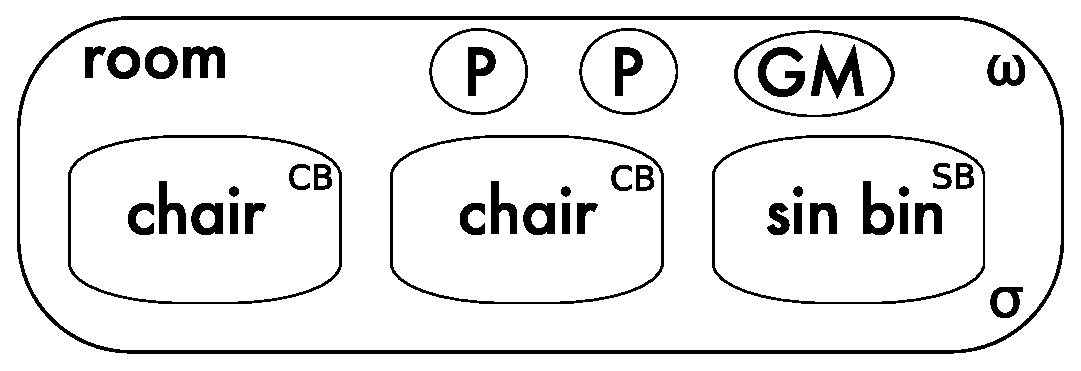
\includegraphics[scale=0.5]{gameenvbw}
  \caption{The Musical Chairs Environment}
  \label{fig:gameenv}
\end{figure}

The environ structure is represented graphically by Fig. \ref{fig:gameenv}
and in the calculus by the equation shown below.
\begin{equation}
\loc{room}{\nloc{chair}{\nil}{CB} \pc \nloc{chair}{\nil}{CB}
\pc \nloc{sin bin}{\nil}{SB} \pc P \pc P \pc GM}{\Omega}{\sigma}
\end{equation}
where $\nloc{m}{E}{F}$ is abbreviated from $\loc{m}{E}{F}{}$.  The
players themselves are represented by \emph{processes}.  This allows
them both to interact and to move between environs.  A gamesmaster
process is also introduced.  This doesn't play an active role in the
game itself, but is instead responsible for performing the
administrative duties of removing chairs from the game and controlling
player movement.  The process definitions are summarised in Table
\ref{tab:musicalchairs}, and make use of the derived syntax for a clock
prefix, $\sigma.P$, shown in \ref{clockcontrol}.

\begin{table}[h]
  \caption{Summary of Processes and Derived Syntax for Musical Chairs}
  \label{tab:musicalchairs}
  \shrule
  \begin{align}
   CB &
    \eqdef 
    \mu X.(\bin.\bout.X + \bopen.\Omega) \label{chairb} \\
   SB &
    \eqdef 
    \mu X.\bin.X \label{sinb} \\
   GM1 &
    \eqdef 
    \sigma.GM2 \label{gmstage2} \\
    GM2 &
    \eqdef 
    \tntopen{chair}.GM3 \label{gmstage3} \\
   GM3 &
   \eqdef
   \sigma.GM4 \label{gmstage4} \\
   GM4 &
    \eqdef  
    \mu X.(\stimeout{\procin{sit}{chair}.X}{\sigma}{GM5}) \label{gmstage5} \\
   GM5 &
    \eqdef 
    \mu X.(\stimeout{\procin{leave}{sinbin}.X}{\sigma}{GM1}) \label{gmstage6}\\
    P &
    \eqdef 
    \sigma.\sigma.MP \label{player} \\
    MP &
    \eqdef
    \stimeout{sit.PIC}{\sigma}{L} \label{mplayer}\\
   PIC &
    \eqdef 
    \sigma.\sigma.PLC \label{pinchair} \\
   PLC &
   \eqdef
   \procout{stand}{chair}.0|stand.P \label{pleavechair} \\
   L &
    \eqdef 
    leave.0 \label{loser} 
  \end{align}
  \shrule
\end{table}

The presence of music is signified by the ticks of a clock, $\sigma$.  A
tick from $\sigma$ is also used to represent the implicit
acknowledgement that everyone who can obtain a chair has done so, and
that the remaining player left in the room has lost.  With regard to the
bouncers of the environs, the room environ is not prone to either
destruction or the entry or exit of other environs, having a bouncer
simply equal to $\Omega$.  This retains the encapsulation of the model
as a single room environ, and prevents other processes or environs
from interfering with its behaviour.

The definition of appropriate bouncers is essential for the chairs
(\ref{chairb}) and the sin bin (\ref{sinb}).  It is the chair bouncer
that enforces the implicit predicate that only one player may inhabit a
chair at any one time, while the sin bin bouncer prevents players
leaving the sin bin once they have entered.

To model stage one of the game, $n$ player processes and $n$ chair
environs are placed in the room.  The advantage of using NT for this
model is that the actual number of players or chairs is irrelevant.
They only have to be equal at the start to accurately model the game.
The calculus allows the creation of a compositional semantics, as
discussed in chapter \ref{introduction}, which works with any $n$.

For the purposes of demonstration, $n$ is assumed to be two to give the
following starting state:
\begin{equation}
  \loc{room}{\nloc{chair}{\nil}{CB} \pc \nloc{chair}{\nil}{CB} \pc 
   P \pc P \pc GM1}{\Omega}{\sigma}.
\end{equation}
The room and chairs appear as shown earlier.  The player
processes (\ref{player}) simply wait until two clock
cycles have passed, the end of each being signalled by a tick from
$\sigma$.  The intermittent period between the ticks (the second clock
cycle) represents the playing of the music.  

Stage two, where the music is started, is thus represented simply by the
first tick of $\sigma$,
\begin{equation}
\begin{aligned}
  & \loc{room}{\nloc{chair}{\nil}{CB} \pc \nloc{chair}{\nil}{CB} \pc 
   P \pc P \pc
   GM1}{\Omega}{\sigma} \\
 \lderives{\sigma}\ & \loc{room}{\nloc{chair}{\nil}{CB} \pc \nloc{chair}{\nil}{CB} \pc 
   \sigma.MP \pc \sigma.MP \pc
   GM2}{\Omega}{\sigma}
\end{aligned}
\end{equation}
which the gamesmaster ($GM1$ (\ref{gmstage2})) also waits for, before
evolving into $GM2$ (\ref{gmstage3}).  The second cycle, prior to the
music stopping, is used to remove a chair from the game.  Maximal
progress, as explained in section \ref{introduction}, ensures that this
occurs before the next clock tick, as the removal emits a high priority
action, $\topen$.  The transition from stage three to stage four is thus
as follows:
\begin{equation}
\begin{aligned}
& \loc{room}{\nloc{chair}{\nil}{CB} \pc \nloc{chair}{\nil}{CB} \pc 
   \sigma.MP \pc \sigma.MP \pc
   GM2}{\Omega}{\sigma} \\
 \lderives{\topen}\ & \loc{room}{\nil \pc \nloc{chair}{\nil}{CB} \pc 
   \sigma.MP \pc \sigma.MP \pc
   GM3}{\Omega}{\sigma}
\end{aligned}
\end{equation}
with one of the two chairs being chosen non-deterministically.
The second tick then occurs, leading in to stage five and the most
interesting part of the model.

\begin{equation}
\begin{aligned}
& \loc{room}{\nil \pc \nloc{chair}{\nil}{CB} \pc 
   \sigma.MP \pc \sigma.MP \pc
   GM3}{\Omega}{\sigma} \\
\lderives{\sigma}\ & \loc{room}{\nil \pc \nloc{chair}{\nil}{CB} \pc 
   MP \pc MP \pc
   GM4}{\Omega}{\sigma} \\
\end{aligned}
\end{equation}

The aim of stage five is to get as many player processes as possible
inside chair environs.  This is handled by again relying on maximal
progress to essentially perform a form of broadcast that centres on
mobile actions, as briefly mentioned in \ref{procmob}.  Rather than
sending a signal to a number of recipients, a request to move into a
chair (see (\ref{gmstage5}) and (\ref{mplayer})) is delivered instead.

If a chair is available, then a player process will enter it (the actual
chair and player chosen is non-deterministic).  This will cause a high
priority action to occur, which takes precedence over the clock tick.
Thus, when the clock eventually does tick, it is clear that no more
players can enter chairs. Using clocks in this manner makes the system
\emph{compositional}; in contrast to other models, players and chairs
can be added without requiring changes to the process definitions.  In
this running example, there are two players, but only one chair, which
results in a single $\tin$ transition:
\begin{equation}
\begin{aligned}
& \loc{room}{\nil \pc \nloc{chair}{\nil}{CB} \pc 
   MP \pc MP \pc
   GM4}{\Omega}{\sigma} \\
\lderives{\tin}\ & \loc{room}{\nil \pc \nloc{chair}{\nil \pc PIC}{\bout.CB} \pc 
   MP \pc
   GM4}{\Omega}{\sigma} \\
\end{aligned}
\end{equation}
that causes one of the $MP$ processes to move in to a
chair, and become a $PIC$ process.  This is followed by the
$\sigma$ transition, which marks the move to stage six.

\begin{equation}
\begin{aligned}
&  \loc{room}{\nil \pc \nloc{chair}{\nil \pc PIC}{\bout.CB} \pc 
   MP \pc
   GM4}{\Omega}{\sigma} \\
\lderives{\sigma}\ & \loc{room}{\nil \pc \nloc{chair}{\nil \pc \sigma.PLC}{\bout.CB} \pc 
   L \pc
   GM5}{\Omega}{\sigma} \\
\end{aligned}
\end{equation}

Both stage six and seven proceed in a similar way.  Stage six sees
essentially the same broadcasting behaviour applied to the losing
players (see (\ref{gmstage6}) and (\ref{loser})).  The difference is
that stage six demonstrates something which wouldn't be possible without
mobility: the broadcast is limited to those player processes which
remain in the room.  As communication between processes in different
environs is disallowed in NT, an implicit scoping of the broadcast
occurs.  In the example, stage six again sees just one $\topen$
transition:
\begin{equation}
\begin{aligned}
&  \loc{room}{\nil \pc \nloc{chair}{\nil \pc \sigma.PLC}{\bout.CB} \pc 
   L \pc
   GM5}{\Omega}{\sigma} \\
\lderives{\topen}\ & \loc{room}{\nil \pc \nloc{chair}{\nil \pc \sigma.PLC}{\bout.CB} \pc
   GM5}{\Omega}{\sigma} \\
\end{aligned}
\end{equation}
which results in the remaining $MP$ (now a losing process, $L$) moving
to the sin bin.  Due to space constraints, the sin bin environ is not
shown in the above derivations.  It may be factored in to the above as
follows:
\begin{equation}
\begin{aligned}
& \nloc{sinbin}{\nil}{SB} \pc L \pc GM5 \\
\lderives{\tin} & \nloc{sinbin}{\nil \pc \nil}{SB} \pc GM5
\end{aligned}
\end{equation}
 where the $L$ process evolves to become a simple $\nil$
process.  The broadcast is again terminated by a tick from $\sigma$,
\begin{equation}
\begin{aligned}
&  \loc{room}{\nil \pc \nloc{chair}{\nil \pc \sigma.PLC}{\bout.CB} \pc
   GM5}{\Omega}{\sigma} \\
\lderives{\sigma}\ & \loc{room}{\nil \pc \nloc{chair}{\nil \pc PLC}{\bout.CB} \pc
   GM1}{\Omega}{\sigma} 
\end{aligned}
\end{equation}
which, in this case, also signifies the music starting up again.  The
remaining players leave their chairs:
\begin{equation}
\begin{aligned}
& \loc{room}{\nil \pc \nloc{chair}{\nil \pc PLC}{\bout.CB} \pc
   GM1}{\Omega}{\sigma}   \\
\lderives{\tout}\ & \loc{room}{\nil \pc \nloc{chair}{\nil \pc \nil}{CB} \pc
   GM1 \pc P}{\Omega}{\sigma} 
\end{aligned}
\end{equation}
and the system essentially returns to the beginning, with $n -
1$ chairs and $n - 1$ players.

\section{A Prototypical Application in NT}
\label{app:nt}

Recall that in \ref{app:req} we specified a series of requirements for a music player application:

\begin{itemize}
\item The application should provide some form of interface with which
  the user can interact.
\item It should be able to take a wave file and return a sequence of
  sound data for playback.
\item It should be able to output the sound data through the speakers.
\item It should be able to generate a spectral analysis of the sound
  data as a form of visual feedback.
\end{itemize}

Now that we have our process calculus to work with, we can provide a formal design for this application,
which can then be converted directly into a real-world application using DynamiTE in the next chapter.

First, we will consider the reading of the wave file.  The simplest solution is:

\begin{equation}
  In \eqdef i.\mu X.\tau.\overline{o}.X
\end{equation}
\noindent where the filename is read in on $i$ and processed to
produce some sound data in the $\tau$ action.  The data is then output
on $o$.  We then recurse, continuing to produce more sound data and
output it on $o$\footnote{At some point, the $\tau$ process will reach
  the end of the file; there isn't an obvious way of representing this
  in the design so we just have to assume that, in the implementation,
  the internal $\tau$ process will terminate the thread running
  $In$.  We could use $X + \nil$ at the end, but then we are
  representing the end of the process as being non-deterministic, when
  it is in fact determined by the file.}.

From this, we can already determine some things about the other processes in the system:

\begin{itemize}
\item The interface ($Intf$) must output on $\overline{i}$ to trigger
  $In$ into starting to produce sound.
\item The speaker output ($Out$) must read on $o$ to obtain the sound
  data and send it to the speakers.
\item The spectral analyser ($Analy$) must read on $o$ to obtain the
  sound data and produce the visual feedback.
\end{itemize}

and definitions for $Out$ and $Analy$ follow fairly
trivally\footnote{We could represent these processes outputting on
  channels representing the speakers and display respectively, but in
  reality these are going to be system calls in the $\tau$ process,
  just as the $\tau$ in $In$ performs reading and decoding
  operations on the file to produce sound data}:

\begin{equation}
\begin{aligned}
  & Out \eqdef o.\tau.\nil \\
  & Analy \eqdef o.\tau.\nil
\end{aligned}
\end{equation}

This already highlights one problem with the current $In$ process.
Both $Out$ and $Analy$ need to synchronise with it on the $o$ channel,
but it currently only performs one $\overline{o}$ action.  Thus, on
each loop within $In$, one of the two will synchronise and the other
will miss out.

From \ref{tpl} and \ref{example}, we already know the best way to
solve this; with a timeout.  $In$ needs to recurse over the
$\overline{o}$ action until it can no longer synchronise with a
receipient, at which point it reads the next piece of sound data; this
is exactly the same logic as we employed for the compositional
broadcast agent in \ref{tpl}.  As a result, $In$ now looks like this:

\begin{equation}
  In \eqdef i.\mu X.\tau.\mu W.\stimeout{\overline{o}.W}{\sigma}{X}
\end{equation}

\noindent We bind $W$ to $\timeout{\overline{o}.W}{\sigma}{X}$ so that
each time $\overline{o}$ is performed, we return to our original state.
When $In$ is running in parallel with $Out$ and $Analy$:

\begin{equation}
  IntSys \eqdef i.\mu X.(\tau.\mu W.\stimeout{\overline{o}.W}{\sigma}{X} \pc o.\tau.\nil \pc o.\tau.\nil)
\end{equation}

\noindent the presence of both $o$ and $\overline{o}$ will allow a
$\tau$ transition to occur (rule $Par2$ in the semantics), which in
turn inhibits $\sigma$.  Once both have occurred, $\sigma$ transitions
can occur and will cause recursion to occur via the expansion of $X$.
Our structural congruence rules ($SCong$) mean that we can simply
discard the two $\nil$ processes left behind by $Out$ and $Analy$.

There is one remaining issue with this construction; the internal
$\tau$ actions of $Out$ and $Analy$ will also cause $In$ to continue
to recurse on $W$ rather than reading the next piece of input.  The
solution to this is to also synchronise these two processes on
$\sigma$:

\begin{equation}
  Out \eqdef o.\stimeout{\Delta}{\sigma}{\tau.\nil}
\end{equation}

\noindent so that now, once input has been received on $o$, $Out$
waits until $\sigma$ becomes unimpeded and is able to tick; $\Delta$
produces no transitions, so neither $STO2$ or $STO3$ can be applied,
and $STO1$ requires the absence of any high priority transitions,
which includes $\tau$ transitions. This should allow all three
processes to continue with their internal processing.  The same
definition can be applied to $Analy$.

Of course, we could provide a much simpler solution by just performing
$\overline{o}$ twice.  The advantage of this solution, as we have
discussed before, is that we can add any number of other processes
that need to synchronise on $o$ without having to alter our definition
of $In$.

All that remains to complete our definition of this system is to
define the interface.  This is simply a means of translating user
actions into calls to our internal system.  This can be as simple as:

\begin{equation}
  Intf \eqdef useri.(\overline{i}.\nil | IntSys)
\end{equation}

But what does $useri$ synchronise with?  This comes from the user and
is outside the system itself:

\begin{equation}
   \procin{begin}{player}.0 \pc begin.\overline{useri}.\nil \pc \loc{player}{Intf}{\bin.\Omega}{\sigma}
\end{equation}

\noindent Our system is now encapsulated in an environ, $player$.  To
start the player, a client must enter $player$ and synchronise on
$useri$.  The bouncer of the $player$ environ allows only one process
to enter, by providing only one $\bin$ with which to synchronise.
$\sigma$ is hidden outside the environ so all the ticks from within
$player$ appear as silent actions to those outside (see $LHd1$).  As
all the other transitions performed by $Intf$ will also be silent
actions, being a mix of internal $\tau$ actions and synchronisations
between $i$ and $o$, processes outside $player$ can use the presence
of these transitions to determine whether or not $Intf$ is active or
not.

We have deliberately kept the design as simple as possible to make it
easier to digest and to reduce the complexity of the corresponding
implementation we will cover in \ref{app:dynamite} as part of our
discussion of DynamiTE.  There are many more things that could be
represented, not the least being a way of stopping playback once
begun!

\section{Conclusion}

In this chapter, we introduced our process calculus, Nomadic Time, the
first novel work in this thesis.  This extends the CaSE process
calculus of chapter \ref{case} with the notions of localities (see
\ref{migration}) and process migration (see \ref{ambientcalculus}).
We also added the notion of `bouncers', a security mechanism which
allows the number and type of mobility operations which may be
performed on an environ (our term for a locality in NT) to be defined.
The first half of the chapter demonstrated how each of these features
was layered on to the calculus, before finishing with its operational
semantics (\ref{ntsemantics}).  We then demonstrate how the calculus
may be used using two examples; the first (\ref{example}) aimed to
demonstrate each of the features of the calculus in action, while the
second (\ref{app:nt}) expanded on the application specified in
\ref{app:req} from a more real-world perspective.

In the next chapter, we show how Nomadic Time may be used to construct
a concurrent programming framework in the Java programming language.
We refer to this framework as the DynamiTE (Dynamic Theory Execution)
framework, and this forms the second novel work in this thesis.  We
then use this framework to implement the prototypical application,
directly using the design from \ref{app:nt} to construct corresponding
Java classes which meet the requirements in \ref{app:req}.  Finally,
we cover some other existing attempts to provide implementations of
process calculi.
